\chapter{Le mouvement rectiligne uniformément accéléré (MRUA)}
Le \motcle{mouvement rectiligne uniformément accéléré} est celui d'un objet se déplaçant en ligne droite et dont la vitesse augmente ou diminue de manière continue.

\section{Étude du MRUA}
Le rail de dynamique permet de créer un MRUA et d'en mesurer facilement les paramètres. Sur ce dispositif, le chariot est entraîné par la masse et sa vitesse augmente de manière constante.
\begin{figure}[h!]
  \centering
  \resizebox{.7\linewidth}{!}{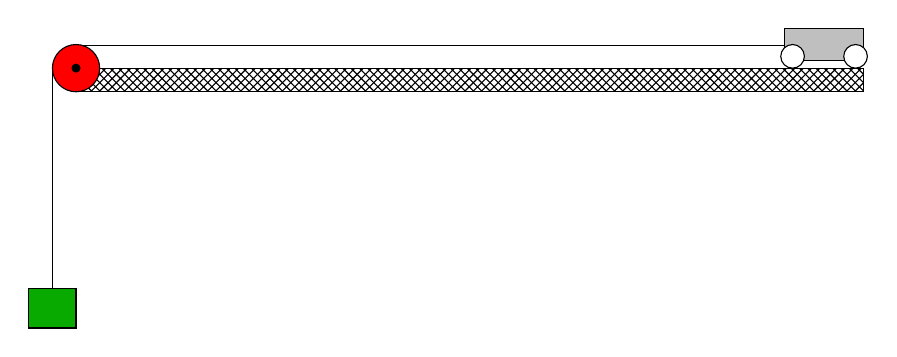
\begin{tikzpicture}
\usetikzlibrary[patterns]
\definecolor{my_green}{HTML} {08aa00}

\node (masse) at (4.7,1.25){};
\node (chariot) at (14.5,4.59){};
\node (poulie_g) at (4.7,4.4){};
\node (poulie_d) at (4.8,4.59){};

\draw (masse) to (poulie_g);%la corde
\draw (poulie_d) to (chariot);%la corde

\filldraw [pattern=crosshatch](5,4) rectangle (15,4.3); %le rectangle du rail
\filldraw[fill=red,draw=black] (5,4.3) circle (3mm);%la poulie
\filldraw[fill=black,draw=black] (5,4.3) circle (0.5mm);%l'axe de la poulie

\filldraw [fill=lightgray,draw=black](14,4.4) rectangle (15,4.8); %le rectangle du chariot
\filldraw[fill=white,draw=black] (14.1,4.45) circle (1.5mm);%roue de gauche
\filldraw[fill=white,draw=black] (14.9,4.45) circle (1.5mm);%roue de droite

\filldraw [fill=my_green,draw=black](4.4,1) rectangle (5,1.5);%rectangle de la masse entrainante



\end{tikzpicture}}
  \caption{Un rail de dynamique}
  \label{rail_dynamique}
\end{figure}
\newpage

\subsection{Graphique et équation horaire de la vitesse}
Le MRUA est un type de mouvement au cours duquel la vitesse augmente ou diminue de manière continue.
\begin{itemize}[label= \textbullet]
  \item Trace, ci-dessous, l'allure du graphique de la vitesse en fonction du temps pour un tel mouvement (vitesse croissante).\\
        \begin{figure}[h!]
          \centering
          \begin{tikzpicture}[>=latex,scale=0.8]
            \tkzInit[xmax=10,ymax=10,xstep=1,ystep=1]
            \tkzGrid[]
            \tkzDrawX[label={$Temps\unit{[s]}$},below left=25pt]
            \tkzDrawY[label={$Vitesse\unit{\unit{[m \cdot s^{-1}]}}$},right=5pt]
            \tkzAxeXY[label={}] %This macro combines the four macros: \tkzDrawX\tkzDrawY \tkzLabelX\tkzLabelY
          \end{tikzpicture}
          \caption{Vitesse en fonction du temps}
          \label{Vitesse en fonction du temps}
        \end{figure}

  \item De quel type de fonction s'agit-il ?
        \pointilles{1}
  \item Écris l'équation correspondante, pense à adapter les symboles utilisés.
        \pointilles{1}
\end{itemize}

\newpage
\subsection{Graphique et équation horaire de l'accélération}
Le graphique ci-dessous présente l'évolution de la vitesse en fonction du temps pour deux mobiles différents.
\begin{itemize}[label=\textbullet]
  \item Quelle est la différence entre les mobiles A et B ?
        %Les élèves doivent constater que la vitesse n'évolue pas au même rythme et que cela correspnd à une différence dans la pente des graphiques
        \pointilles{4}

        \begin{figure}[h!]
          \centering
          \resizebox{.7\linewidth}{!}{\begin{tikzpicture}[>=latex]
\tkzInit[xmax=10,ymax=10,xstep=1,ystep=1]
\tkzGrid[]
\tkzDrawX[label={$Temps[s]$},below left=25pt]
\tkzDrawY[label={$Vitesse[m \cdot s^{-1}]$},right=5pt]
\tkzAxeXY[label={}] %This macro combines the four macros: \tkzDrawX\tkzDrawY \tkzLabelX\tkzLabelY

\tkzDefPoints{0/2/O, 10/6/A, 8/10/B}
\tkzDrawSegment[blue](O,A)
\tkzDrawSegment[red](O,B)
\tkzLabelSegment[color=blue,above=5pt](O,A){$A$}
\tkzLabelSegment[color=red,above=3pt](O,B){$B$}
\end{tikzpicture}
}
          \caption{Deux mobiles en MRUA}
          \label{graph_v1_v2}
        \end{figure}

  \item Que peux-tu en conclure ?
        %la pente du graphique de la vitesse correspond au taux de variation de cette vitesse
        %cette pente est constante
        \pointilles{2}
\end{itemize}

\begin{encadre}
  L' \motcle{accélération} décrit la façon dont la vitesse varie au cours du temps, comme pour la vitesse, il est possible de calculer une valeur de l'\motcle{accélération moyenne} en faisant :
  \( a_{moy} =\frac{\Delta v}{\Delta t} \) ou \(a_{moy} =\frac{v_2 - v_1}{t_2 - t_1} \)
\end{encadre}

\begin{itemize}[label=\textbullet]
  \item Quelles sont les unités S.I. de l'accélération ?
        \pointilles{2}
  \item Trace, ci-dessous, l'allure du graphique de l'accélération en fonction du temps(vitesse croissante).\\
        \begin{figure}[h!]
          \centering
          \begin{tikzpicture}[>=latex,scale=0.8]
            \tkzInit[xmax=10,ymax=10,xstep=1,ystep=1]
            \tkzGrid[]
            \tkzDrawX[label={\(Temps\unit{[s]}\)},below left=25pt]
            \tkzDrawY[label={\(Acc\acute{e}l\acute{e}ration\unit{[m \cdot s^{-2}]}\)},right=5pt]
            \tkzAxeXY[label={}] %This macro combines the four macros: \tkzDrawX\tkzDrawY \tkzLabelX\tkzLabelY
          \end{tikzpicture}
          \caption{Accélération en fonction du temps}
          \label{Accélération en fonction du temps}
        \end{figure}

  \item De quel type de fonction s'agit-il ?
        \pointilles{1}
  \item Écris l'équation correspondante, pense à adapter les symboles utilisés.
        \pointilles{1}
\end{itemize}

\subsection{Graphique et équation horaire de la position}
Nous avons vu que l'équation horaire de l'accélération est de degré \enquote{0} tandis que celle de la vitesse est de degré \enquote{1}.
Il est donc logique que celle de la position soit du deuxième degré.
Celle-ci est donnée par :
\(x(t)=x_0+v_0 \cdot \Delta t + \frac{a}{2} \cdot \Delta t^2\)

Trace, ci-dessous, l'allure du graphique de la position en fonction du temps (vitesse croissante).\\
\begin{figure}[h!]
  \centering
  \begin{tikzpicture}[>=latex,scale=0.8]
    \tkzInit[xmax=10,ymax=10,xstep=1,ystep=1]
    \tkzGrid[]
    \tkzDrawX[label={\(Temps\unit{[s]}\)},below left=25pt]
    \tkzDrawY[label={\(Position[m]\)},right=5pt]
    \tkzAxeXY[label={}] %This macro combines the four macros: \tkzDrawX\tkzDrawY \tkzLabelX\tkzLabelY
  \end{tikzpicture}
  \caption{Position en fonction du temps}
  \label{Position en fonction du temps}
\end{figure}

\newpage

\section{Analyse de cas : la décélération}
Jean est sur son vélo, il roule à la vitesse de 14,4\unit{[km/h]} et se déplace dans le sens croissant du référentiel. Un chien traverse la route devant lui et Jean serre ses freins jusqu'à ce qu'il s'arrête.
\begin{itemize}[label=\textbullet]
  \item À partir du moment où il freine, comment varie la position de Jean ?
        \pointilles{2}
  \item Comment varie sa vitesse ?
        \pointilles{2}
  \item Comment varie son accélération, que vaut-elle ?
        \pointilles{2}

  \item Si on considère que son mouvement est décrit par un MRUA, trace l'allure du graphique de la position en fonction du temps, de la vitesse en fonction du temps et de l'accélération en fonction du temps.
\end{itemize}

\newpage
\section{Synthèse}
\subsection{Équations horaires du MRUA}

\begin{encadre}
  Position\\
  \(x(t)=x_0+v_0 \cdot \Delta t + \frac{a}{2} \cdot \Delta t^2\)
\end{encadre}

\begin{encadre}
  Vitesse\\
  \(v(t)=v_0+a \cdot \Delta t\)
\end{encadre}

\begin{encadre}
  Accélération \\
  \(a=cst\)
\end{encadre}

\subsection{Graphiques types du MRUA}
Les graphiques ci-dessous sont toujours ceux d'un mobile progressant dans le sens croissant du référentiel.

\begin{tabularx}{\linewidth}{m{.1\linewidth} X X X}
  \hline
                       & Position en fonction du temps & Vitesse en fonction du temps & Accélération en fonction du temps \\
  \hline
  \rotatebox{90}{MRUA} &                               &                              &                                   \\[4cm]
  \hline
  \rotatebox{90}{MRUD} &                               &                              &                                   \\[4cm]
  \hline \hline
\end{tabularx}
\section{Exercices}
\begin{exercise}
  Une Opel Corsa 5 1.4 est à l'arrêt sur une piste de course. Un chronomètre est en fonctionnement. Lorsqu'il indique 33\unit{[s]}, la voiture commence à accélérer et lorsqu'il indique 44\unit{[s]}, elle a atteint la vitesse de 100\unit{[km/h]}. Si on suppose que l'accélération est constante, calcule celle-ci en unités SI.
\end{exercise}
\begin{solution}
  \(a=2,525\unit{[m \cdot s^{-2}]}\)
\end{solution}
\begin{exercise}
  Lors d'une démonstration, la Mercedes AMG F1W03 pilotée par Anthony Davidson a atteint la vitesse de 200 \unit{[km/h]} en 5,7 secondes. Si on suppose que l'accélération est constante, calcule celle-ci en unités SI.
\end{exercise}
\begin{solution}
  \(a=9,747\unit{[m \cdot s^{-2}]}\)
\end{solution}

\begin{exercise}
  Un objet qui, à la surface de la Terre, tombe d'une hauteur de 100[m] arriverait au sol 4,515 secondes plus tard avec une vitesse de 44,2945 m/s s'il n'y avait pas de frottements avec l'air. Calcule accélération de cet objet. À quoi correspond-elle ?
\end{exercise}
\begin{solution}
  \(a=9,81\unit{[m \cdot s^{-2}]}\), il s'agit de l'accélération de la pesenteur terrestre : g.
\end{solution}

\begin{exercise}
  Une voiture part du repos, accélère de manière constante puis, lorsqu'elle a atteint la vitesse souhaitée, continue à vitesse constante.
  Trace l'allure des graphiques de la position, de la vitesse et de l'accélération en fonction du temps pour cette situation.
\end{exercise}

\begin{exercise}
  Un vélo roule à vitesse constante. Lorsqu'il rencontre un obstacle, il freine jusqu'à l'arrêt complet.
  Trace les graphiques de la position, de la vitesse et de l'accélération en fonction du temps pour cette situation.
\end{exercise}

\begin{exercise}
  Un homme saute à l'élastique depuis un pont. Il commence par tomber en chute libre avec une accélération constante puis l'élastique commence à se tendre et il subit une décélération constante. Trace les graphiques de la position, de la vitesse et de l'accélération en fonction du temps pour cette situation entre le moment où il saute et celui où il atteint son point le plus proche du sol.
\end{exercise}

\begin{exercise}
  Le graphique ci-dessous est celui de la vitesse en fonction du temps pour un mobile.
  \begin{enumerate}[label=\alph*)]
    \item Trace un graphique plausible pour la position et l'accélération en fonction du temps.
    \item Crée un scénario plausible.
          \begin{figure}[h!]
            \centering
            \begin{tikzpicture}[>=latex,scale=0.5]
              \tkzInit[xmax=10,ymax=10,xstep=1,ystep=1]
              \tkzGrid[]
              \tkzDrawX[label={\(Temps\unit{[s]}\)},below left=25pt]
              \tkzDrawY[label={\(Vitesse\unit{[m \cdot s^{-1}]}\)},right=5pt]
              \tkzAxeXY[label={}] %This macro combines the four macros: \tkzDrawX\tkzDrawY \tkzLabelX\tkzLabelY
              \tkzDefPoints{0/5/O,3/5/A,6/2/B,10/2/C}
              \tkzDrawSegments[ultra thick,color=red](O,A A,B B,C)
            \end{tikzpicture}
            \caption{Vitesse en fonction du temps}
            \label{Vitesse en fonction du temps}
          \end{figure}
  \end{enumerate}
\end{exercise}


\begin{exercise}
  Le graphique ci-dessous est celui de la position en fonction du temps pour un mobile.
  \begin{enumerate}[label=\alph*)]
    \item Que peux-tu dire concernant la vitesse initiale de ce mobile ?
    \item Que vaut sa vitesse après 4 secondes ?
    \item Que peux-tu dire concernant sa vitesse finale ?
    \item Que peux-tu dire concernant son accélération ?
          \begin{figure}[h!]
            \centering
            \begin{tikzpicture}[>=latex,scale=0.5]
              \tkzInit[xmax=10,ymax=10,xstep=1,ystep=1]
              \tkzGrid[]
              \tkzDrawX[label={\(Temps\unit{[s]}\)},below left=25pt]
              \tkzDrawY[label={\(Position[m]\)},right=5pt]
              \tkzAxeXY[label={}] %This macro combines the four macros: \tkzDrawX\tkzDrawY \tkzLabelX\tkzLabelY
              \tkzFct[domain =0:8,ultra thick,color=red]{-(0.5*x-2)**(2)+5} %
            \end{tikzpicture}
            \caption{Position en fonction du temps}
            \label{Position en fonction du temps}
          \end{figure}
  \end{enumerate}
\end{exercise}

\begin{exercise}
  Une voiture accélère de 43,2 \unit{[km/h]} à 93,6\unit{[km/h]} en 6\unit{[s]}.
  \begin{enumerate}[label=\alph*)]
    \item Quelle est son accélération ?
    \item Quelle est la distance parcourue durant ce temps ?
  \end{enumerate}
\end{exercise}
\begin{solution}
  \(a=2,333\unit{[m \cdot s^{-2}]} ; \Delta x=114[m] \)
\end{solution}


\begin{exercise}
  Une voiture ralenti et sa vitesse passe de accélère de 111,6 \unit{[km/h]} à 46,8\unit{[km/h]} en 12\unit{[s]}.
  \begin{enumerate}[label=\alph*)]
    \item Quelle est son accélération ?
    \item Quelle est la distance parcourue durant ce temps ?
  \end{enumerate}
\end{exercise}
\begin{solution}
  \(a=-1,5\unit{[m \cdot s^{-2}]} ; \Delta x=264[m]\)
\end{solution}

\begin{exercise}
  Un avion à réaction doit atteindre la vitesse de 80\unit{[m/s]} pour décoller sur une piste de 1500[m] de long.
  \begin{enumerate}[label=\alph*)]
    \item Quelle doit être son accélération ?
    \item Combien de temps cela prend-il ?
  \end{enumerate}
\end{exercise}
\begin{solution}
  \(a=2,133\unit{[m \cdot s^{-2}]} ; \Delta t=37,5\unit{[s]}\)
\end{solution}

\begin{exercise}[difficulty=**]
  Un train mesurant 75[m] de long se met en marche et accélère uniformément. La locomotive croise un employé de chemin de fer à 140[m] de son point de départ à la vitesse de 25\unit{[m/s]}, quelle est la vitesse du train lorsque que le dernier wagon passe devant cet employé ?
\end{exercise}

\begin{exercise}
  Un mobile se déplace à vitesse constante lorsqu'il passe devant une personne qui enclenche un chronomètre. Lorsque le chronomètre indique \(323\unit{[s]}\), le mobile commence à accélérer. Son accélération vaut : \(a=0,6\unit{[m \cdot s^{-2}]}\) et il atteint la vitesse de \(\num{1325,6}\unit{[m \cdot s^{-1}]}\) lorsque le chronomètre indique \(\num{2518}\unit{[s]}\). Quelle était la vitesse de départ de ce mobile?
\end{exercise}



\begin{exercise}
  Un mobile se déplace avec une vitesse égale à \(v_0=9,2\unit{[m \cdot s^{-1}]}\) lorsqu'il commence à accélérer. Son accélération vaut \(a=0,28\unit{[m \cdot s^{-2}]}\) et sa position \(212\unit{[s]}\) plus tard vaut \(x=\num{10542,56}[m]\).
  Quelle était la position initiale du mobile ?
\end{exercise}


\begin{exercise}
  Un mobile se déplace avec une vitesse initiale égale à \(v_0=8,3\unit{[m \cdot s^{-1}]}\).
  Lorsque sa position vaut \(x=2700[m]\), il commence à accélérer. Son accélération vaut \(a=0,27\unit{[m \cdot s^{-2}]}\).
  Quelle est la position de ce mobile \(136\unit{[s]}\) plus tard ?
\end{exercise}



\begin{exercise}
  Pendant combien de temps un mobile doit-il accélérer pour que sa vitesse atteigne \(133,3\unit{[m \cdot s^{-1}]}\). Sa vitesse de départ vaut : \(v_0=7,5\unit{[m \cdot s^{-1}]}\) et son accélération : \(a=0,1\unit{[m \cdot s^{-2}]}\).
\end{exercise}


\begin{exercise}
  Un mobile se déplace avec une vitesse initiale égale à \(v_0=5,9\unit{[m \cdot s^{-1}]}\). Il commence à accélérer. Son accélération vaut \(a=2,6\unit{[m \cdot s^{-2}]}\).
  Quelle est la vitesse de ce mobile \(1677\unit{[s]}\) plus tard?
\end{exercise}

\begin{exercise}
  Un mobile se déplace à la vitesse constante de \(v=9,9\unit{[m \cdot s^{-1}]}\), lorsque sa position vaut \(x_1=1900[m]\), il commence à accélérer. Sa position \(1016\unit{[s]}\) plus tard vaut \(x_2=\num{1353891,2}[m]\).
  Quelle était l'accélération du mobile?
\end{exercise}

\begin{exercise}
  Un mobile se déplace à vitesse constante, lorsque sa position vaut \(2600[m]\), il commence à accélérer.
  Son accélération vaut \(a=0,8[m \cdot s^{-2}]\) et sa position \(2557\unit{[s]}\) plus tard vaut \(x=\num{2631451,7}[m]\).
  Quelle était la vitesse initiale du mobile ?
\end{exercise}

\begin{exercise}
  Un mobile se déplace avec une vitesse initiale égale à \(v_0=9,9[m \cdot s^{-1}]\). Lorsque sa position vaut \(x=2800[m]\), il commence à freiner. Son accélération vaut \(a=-1,7[m \cdot s^{-2}]\).
  \begin{enumerate}[label=\alph*)]
    \item Combien de temps prend-il pour s'arrêter?
    \item Quelle distance prend-il pour s'arrêter?
  \end{enumerate}
\end{exercise}

\begin{exercise}
  Un mobile se déplace à la vitesse constante de \(6,4[m \cdot s^{-1}]\), lorsque sa position vaut \(x_1=1200[m]\), il commence à accélérer jusqu'à atteindre la position de \(x_2=2788,44[m]\). Son accélération vaut \(a=0,62\unit{[m \cdot s^{-2}]}\).
  Pendant combien de temps le mobile a-t-il accéléré ?
\end{exercise}

\begin{exercise}[difficulty=***]
  Une voiture se déplace à 140,4\unit{[km/h]} sur une autoroute lorsqu'elle passe devant une voiture de police roulant à 95,4\unit{[km/h]}. Une seconde plus tard, la voiture de police commence à accélérer avec une valeur de \(a=2\unit{[m \cdot s^{-2}]}\).
  \begin{enumerate}[label=\alph*)]
    \item Combien de temps après le dépassement la voiture de police rattrape-t-elle le chauffard ?
    \item Quelle est la distance parcourue par les deux voitures entre le premier et le deuxième dépassement ?
    \item Quelle est la vitesse de la voiture de police lorsqu'elle attrape-t-elle le chauffard ?
  \end{enumerate}
\end{exercise}

\begin{exercise}[difficulty=***]
  Une voiture se déplace trop vite sur une autoroute lorsqu'elle passe devant une voiture de police roulant à 95,4\unit{[km/h]}. Une seconde plus tard, la voiture de police commence à accélérer avec une valeur de \(a=2\unit{[m \cdot s^{-2}]}\) et 6\unit{[s]} après le dépassement, la voiture de police rattrape le chauffard.
  Quelle était la vitesse de celui-ci ?
\end{exercise}

